% !TEX encoding = UTF-8
% !TEX TS-program = pdflatex
% !TEX root = ../tesi.tex

%**************************************************************
\chapter{Progettazione}
\label{cap:progettazione}
%**************************************************************

\intro{Questo capitolo illustra le caratteristiche dell'applicazione già esistente e lo studio eseguito per comprenderle e motivare le progettuali adottate nello sviluppo del prototipo da me realizzato durante l'esperienza di stage.}\\ %TODO oppure illustra lo stato dell'applicazione

\section{Architettura preesistente}
Trattandosi di effettuare la reimplementazione di una funzionalità preesistente, il primo ostacolo è stato quello di capire come il mio prodotto dovesse integrarsi con il resto dell'architettura cui avrebbe fatto parte, per questo motivo la prima settimana di stage è stata dedicata quasi esclusivamente alla conoscenza dell'ambiente e delle componenti. \\

\subsection{Visione generale}

\begin{figure}[h]
	\centering
	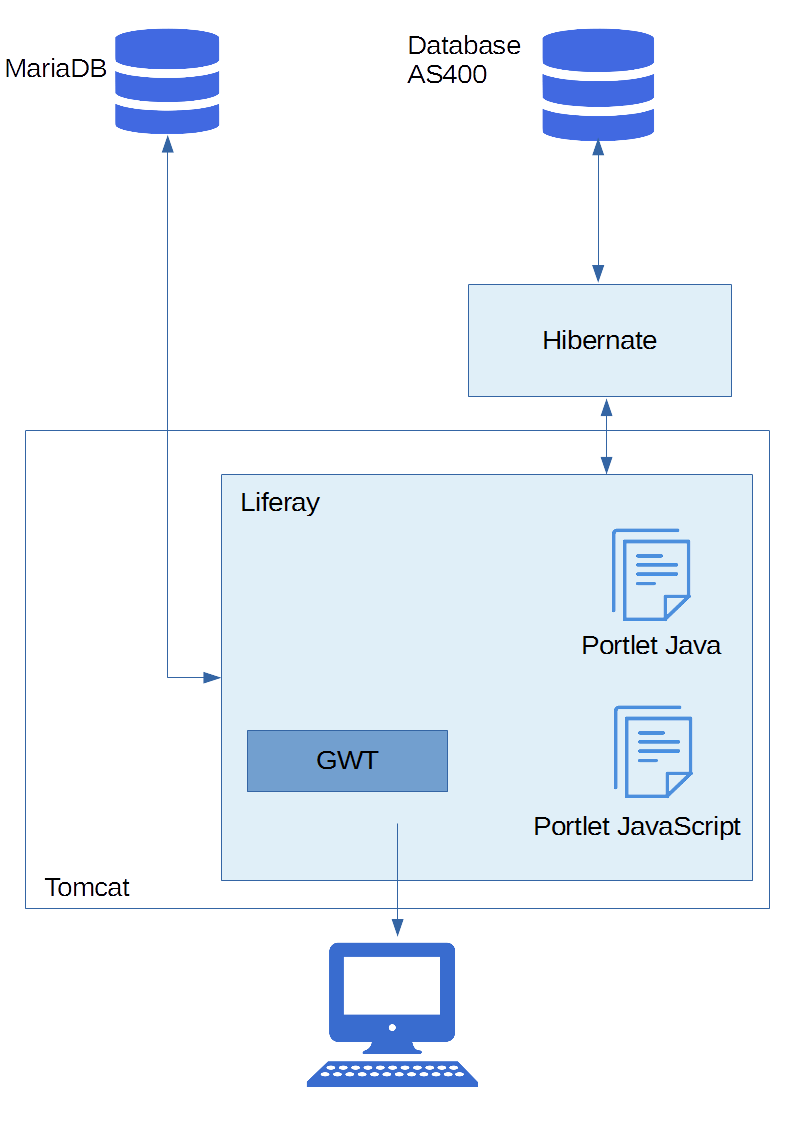
\includegraphics[height = 12 cm]{schema-generale}
	\caption{Schema generale di interconnessione tra le componenti}
	\label{schema-generale}
\end{figure}
la figura \ref{schema-generale} illustra, ad alto livello, le relazioni che intercorrono tra le varie tecnologie utilizzate dal software JGalileo CRM.\\
Partendo dalle basi di dati fino ad arrivare all'interfaccia utente, l'architettura del sistema si snoda nel seguente modo:\\
Entrambe le basi di dati, sia quella contenuta nel database del sistema operativo AS400 che quella contenuta sul server, si interfacciano con il Framework Hibernate per creare delle classi, equivalenti alle tabelle del database, con cui permettere l'interazione.\\ 
La sezione dell'appendice ~\ref{sec:appendice-1} riporta più nel dettaglio come vengono create le entità Hibernate.\\
L'interazione con le entità di Hibernate avviene per mezzo di Liferay, che si occupa anche della gestione degli accessi degli utenti alla pagina, introducendo il concetto di Single Sing On, e della corretta visualizzazione delle \gls{portlet} all'interno delle pagine del portale. Queste sono caricate di volta in volta, tramite dei servizi REST, dal server Tomcat e possono essere scritte in AngularJS, come ad esempio la \gls{portlet} per la geolocalizzazione o quella che gestisce la timeline, oppure in Java per essere successivamente tradotte in JavaScript tramite i servizi offerti da GWT.\\
Le azioni dell'utente vengono gestite poi da Liferay, che si occupa anche del routing tra le varie pagine del portale. Nel caso ci fossero dei dati da salvare, come nel caso dell'inserimento di un nuovo lead, vengono lanciati dei servizi REST che andranno ad interfacciarsi con le entità gestite da Hibernate, il quale gestisce la persistenza dei dati.\\

\subsection{Portlet life cycle}
Al fine di capire al meglio come progettare la nuova form, mi sono concentrato sullo studio del ciclo di vita di una \gls{portlet}:\\
L'ambiente in cui una essa viene creata ed utilizzata è denominato \emph{portlet container} che, come suggerisce la parola, è un contenitore che gestisce l'aggregazione tra le \gls{portlet}, mantiene memoria delle preferenze dettate dall'utente su di esse ed inoltre funge da \emph{Controller} tra l'interfaccia utente(\emph{View}) ed i dati (\emph{Model}) nel paradigma di programmazione MVC (Model View Controller), illustrato nella sezione ~\ref{sec:MVC}.\\

\begin{figure}[h]
	\centering
	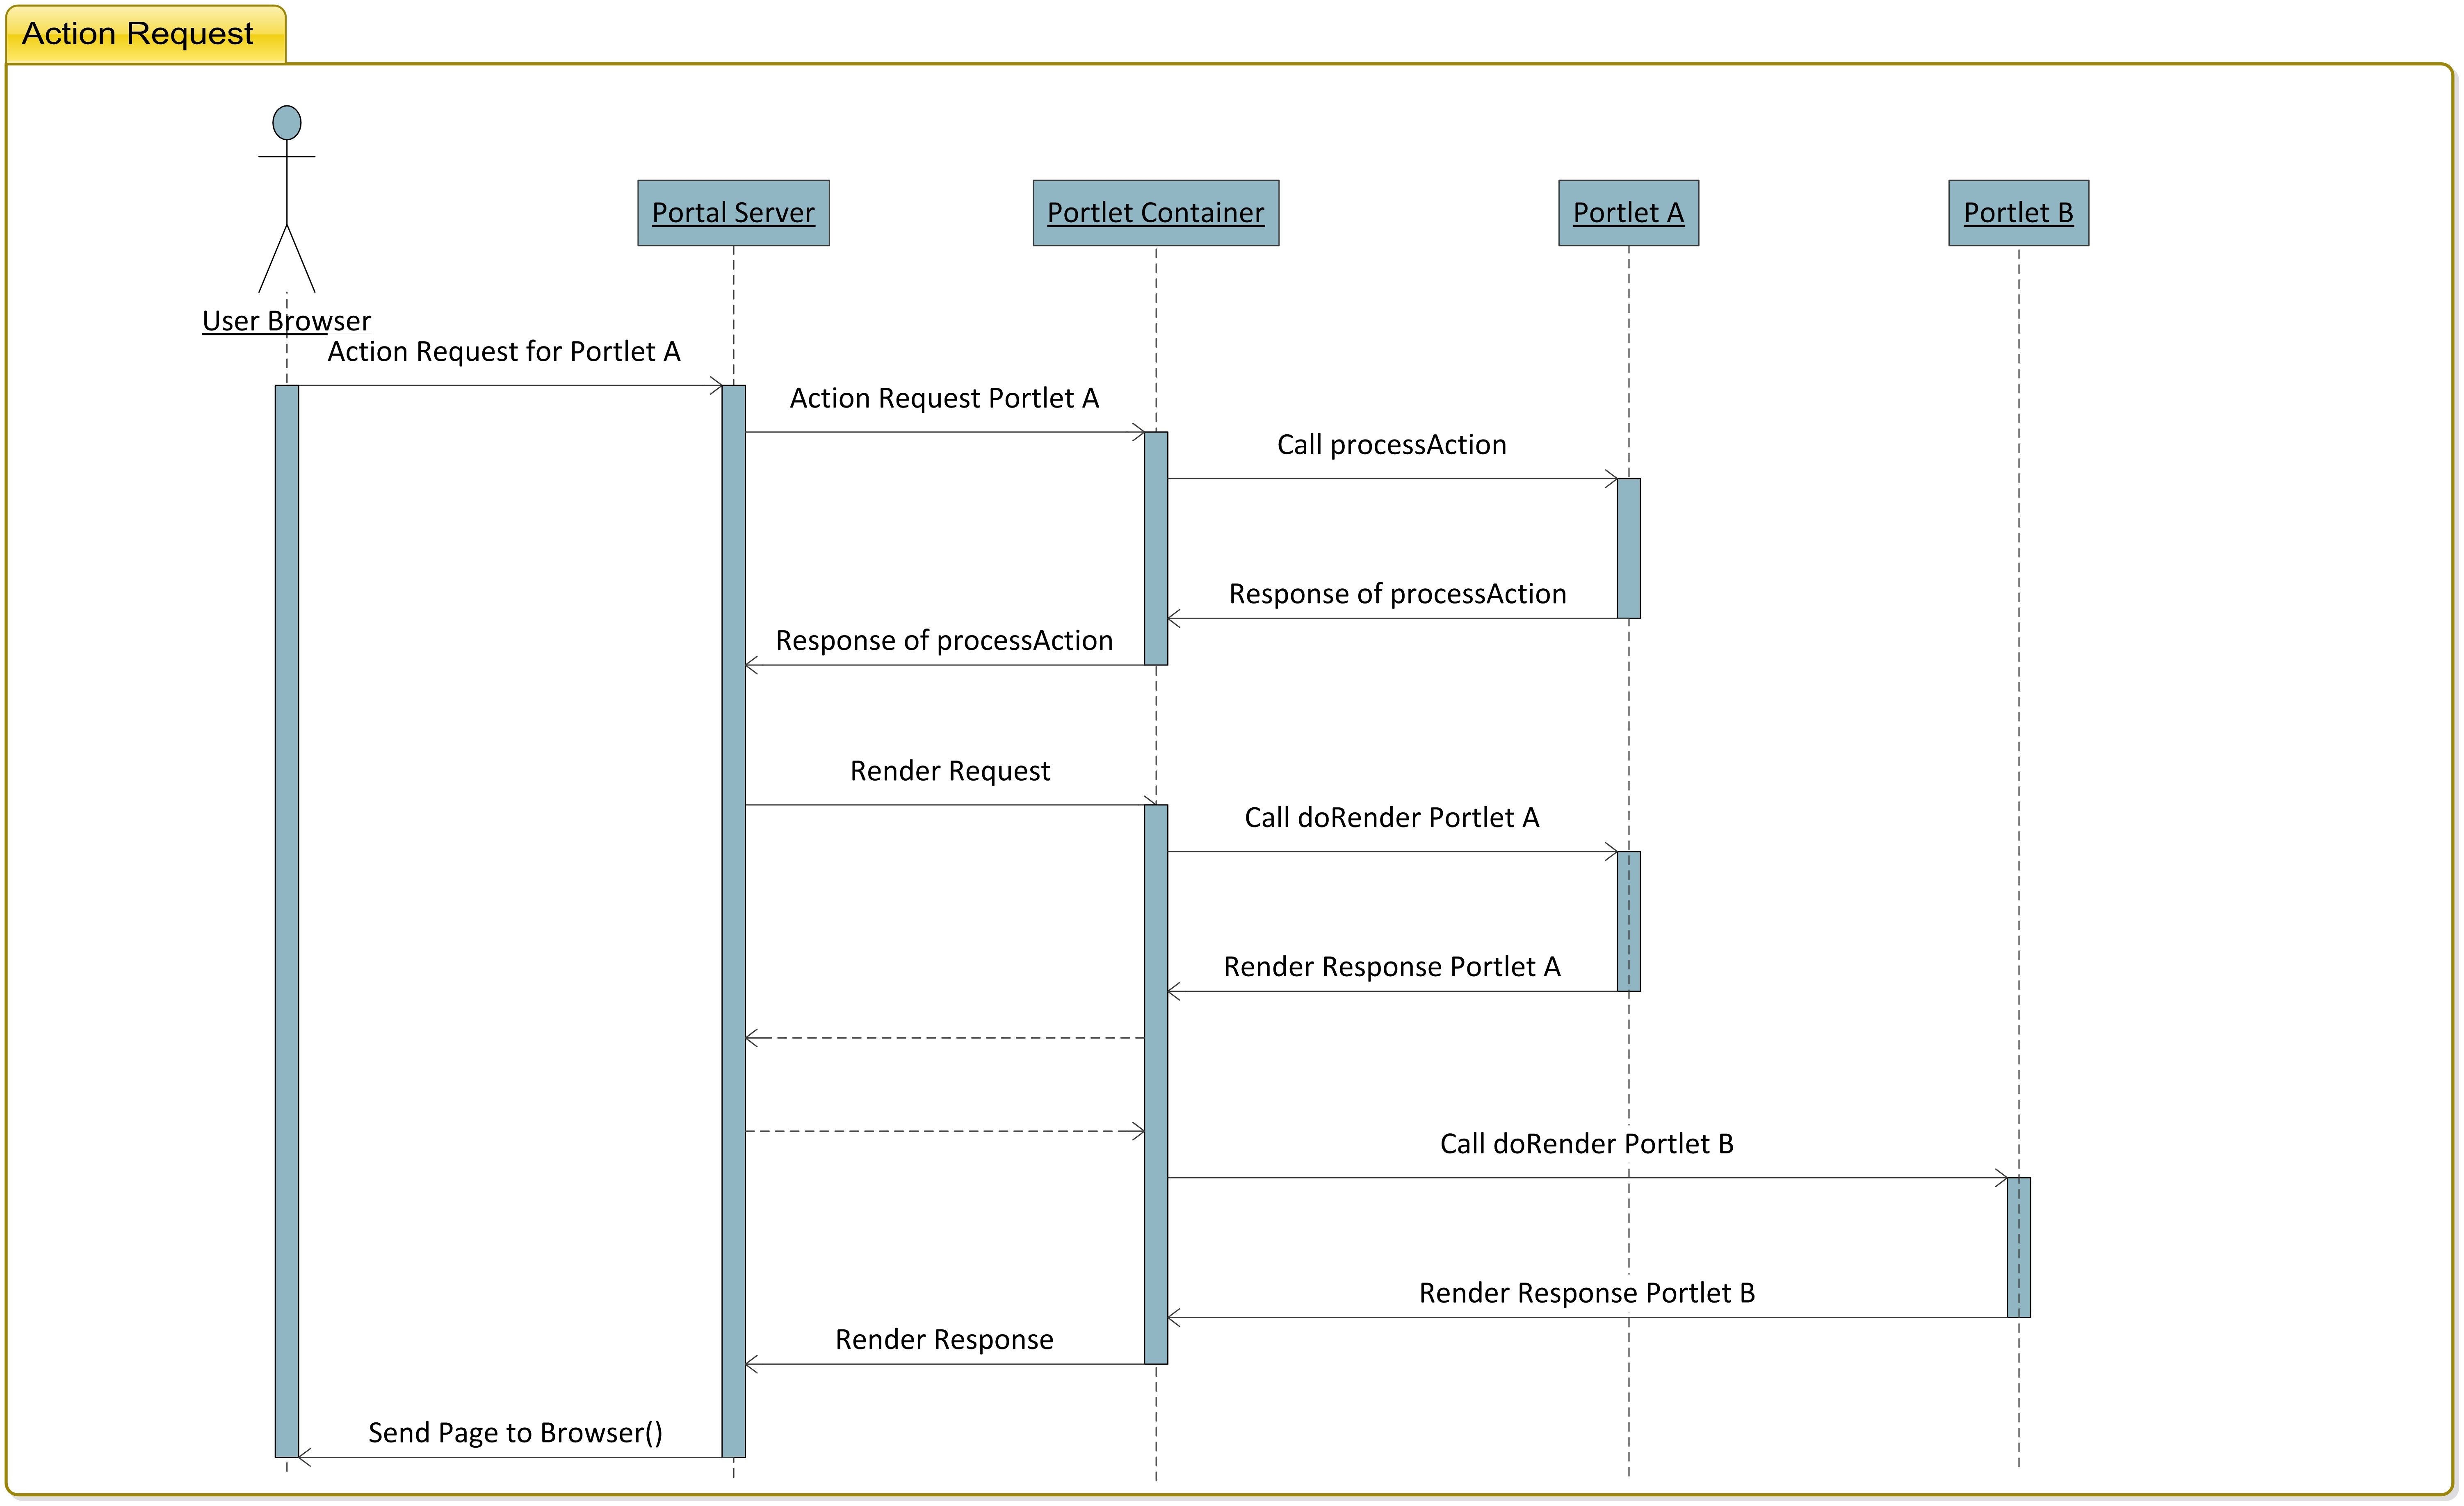
\includegraphics[height = 8 cm]{portet_action_request}
	\caption{Diagramma di sequenza di ProcessAction}
	\label{process-action}
\end{figure}

Il ciclo di vita di una \gls{portlet} è caratterizzato da 6 metodi principali che lo regolano:
\begin{itemize}
	\item \textbf{init()}: chiamato dal portlet container, questo metodo crea la \gls{portlet} desiderata. Durante il ciclo di vita della stassa viene invocato una sola volta;
	\item \textbf{render()}: questo metodo è responsabile della generazione di codice HTML che sarà quindi visualizzato a schermo. Ci sono alcune restrizioni di sicurezza, viene impedita ad esempio la generazione di tag quali <html>, <head>, <body>, che andrebbero a rompere l'intera pagina.
	\item \textbf{processAction()}: processAction viene invocato quando viene eseguita un'azione, ad esempio l'azione di salvataggio di una form. dopo processAction viene automaticamente invocato il metodo render() della portlet e delle altre \gls{portlet}, qualora ve ne fossero.
	\item \textbf{processEvent()}: utilizzato per gestire gli eventi, viene poi chiamato il metodo render() della sola \gls{portlet} interessata;
	\item \textbf{serveRescource()}: metodo utilizzato per reperire risorse utilizzando un \gls{urlg};
	\item \textbf{destroy()}: distrugge la \gls{portlet};
\end{itemize}	

\section{Form portlet}
La form che avrei dovuto reimplementare consiste in un unica portlet,scritta in Java. \\
La portlet è costituita da una grande classe, di oltre 6.000 linee di codice, che si appoggia poi ad altre classi per la gestione di aspetti più particolari: ad esempio i campi di tipo picker, cioè dei campi di ricerca che recuperano le voci su cui effettuarla dal database, è separata e lunga circa 4.000 linee di codice.\\
Data l'estrema lunghezza, in rapporto alla mia esperienza di studente, ed alla mancanza di documentazione dovuta all'adozione della metodologia agile, lo studio del funzionamento della portlet che gestisce la form ha richiesto più tempo del previsto. \\ 
L'analisi ha portato allo sviluppo del diagramma di flusso illustrato nella figura \ref{form-portlet-flow-diagram}, diagramma molto generale a causa della grande complessità di metodi e casistiche dettate dal fatto che la form viene creata dinamicamente e quindi deve coprire tutte le possibili casistiche in cui è possibile incorrere.\\

\begin{figure}[p]
	\centering
	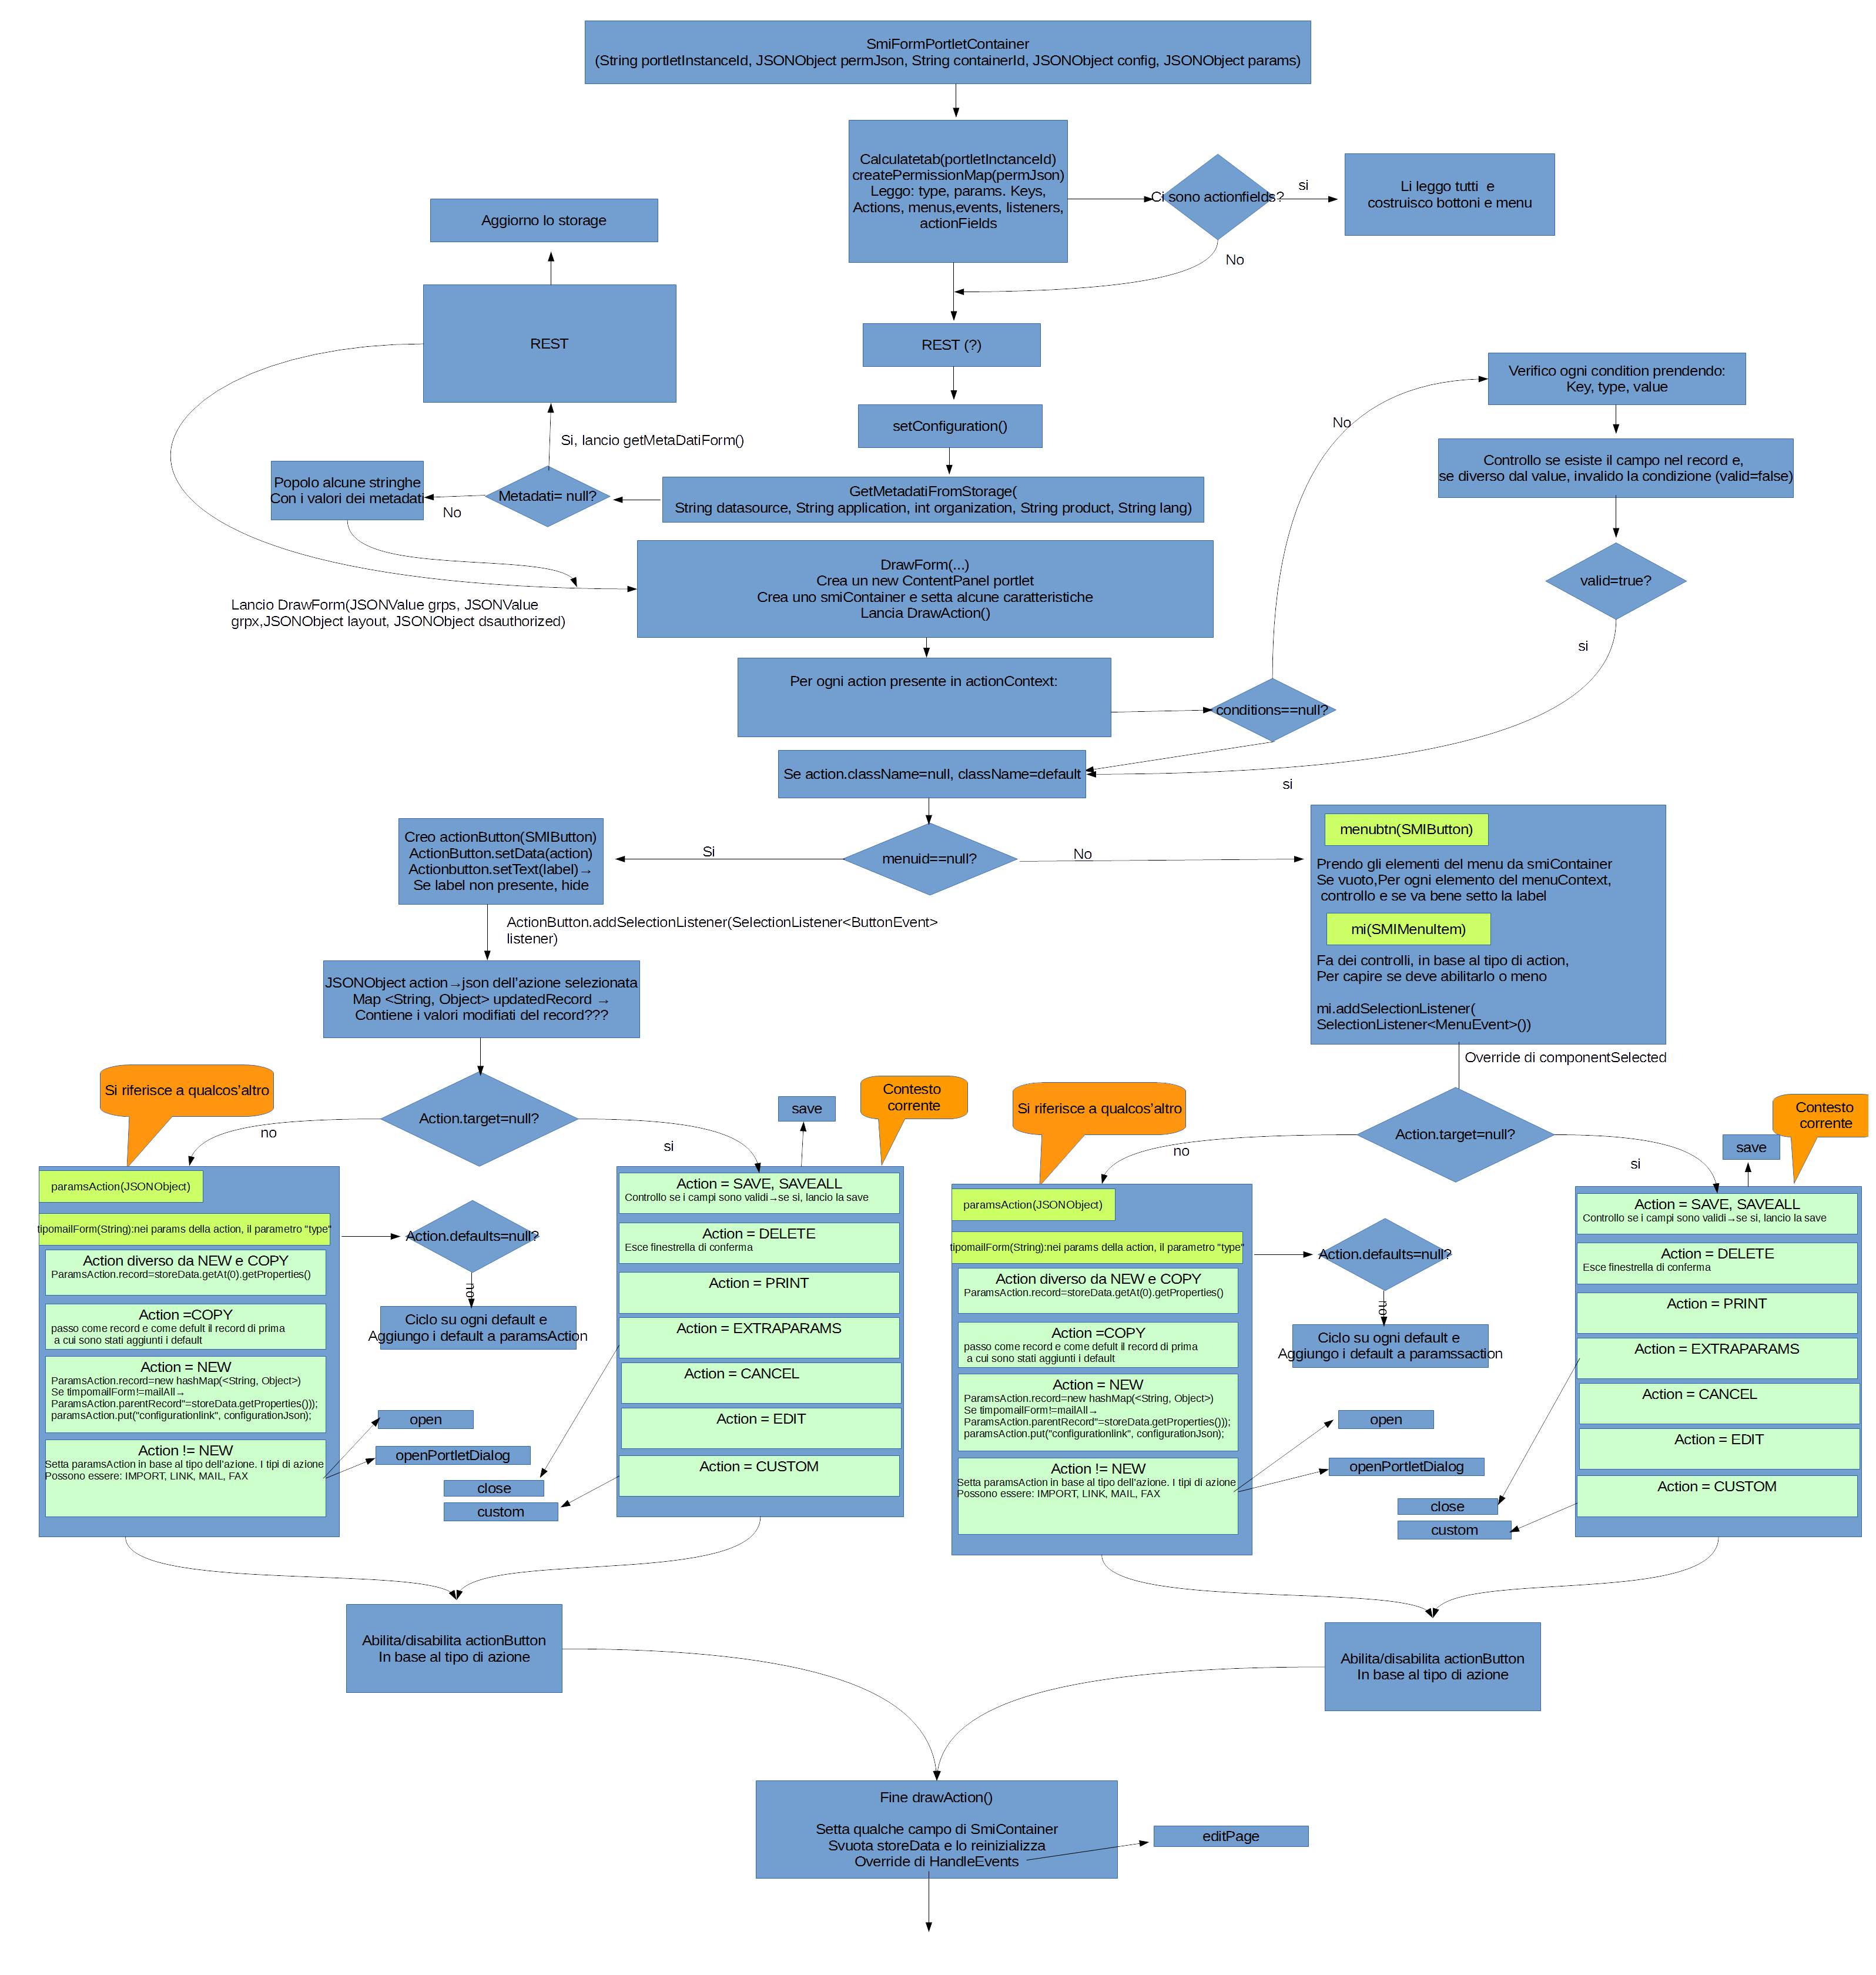
\includegraphics[width=\textwidth, height=\textheight]{diagramma-flusso}
	\caption{Diagramma di flusso della form preesistente}
	\label{form-portlet-flow-diagram}
\end{figure}	